\section{Adaptive Sampling Strategy}
	
\subsection*{Discussion about Random Sampling Stragtegy}
\begin{frame}{Discussion about Randomly Sampling}
	\begin{itemize}
		\setlength{\itemsep}{1.5em}
		\item For a given training sample $\left(u,i,j\right) \in D_s$, the stochastic gradient of an arbitrary parameter $\theta \in \Theta$ is:
		
		\scalebox{0.8}{
			\parbox{1.2\textwidth}{
				\vspace{1em}
				\begin{equation}
				\label{eq19}
				\frac {\partial L_{feedback}} {\partial\theta} 
				= -f\left(-r_{uij}\right)\frac{\partial\left(r_{uij}\right)}{\partial\theta}
				= \left(f\left(r_{uij}\right)-1\right) \frac{\partial\left(r_{uij}\right)}{\partial\theta}
				\end{equation}
			}
		}
		
		
		\item The massive training samples are inefficient to SGD.
		
		\begin{columns}
			\column{3cm}
			\begin{figure}
				\vspace{1em}
				
\includegraphics[width=1in]{man}
			\end{figure}
			\column{4cm}
			\begin{figure}
				\vspace{1em}
				
\includegraphics[width=1.5in,height=1in]{iPhone}
			\end{figure}
			\column{4cm}
			\begin{figure}
				\vspace{1em}
				
\includegraphics[width=1.5in,height=1in]{toothbrush}
				
			\end{figure}
			
		\end{columns}
		\vspace{1em}
	
	\end{itemize}
	
\end{frame}

\subsection*{Overview}


\begin{frame}
	\frametitle{how to select a reasonable negative item $v_j$ ?}
	\vspace{-2em}
	\begin{columns}
		\column{3cm}
		\begin{figure}
			
\includegraphics[width=1in]{man}
		\end{figure}
		\column{3cm}
		\begin{figure}
			
\includegraphics[width=1.5in,height=1in]{iPhone}
		\end{figure}
		\column{4cm}
		\begin{figure}
			
\includegraphics[width=.8in,height=1.5in]{Samsung}
		\end{figure}
	\end{columns}
	\vspace{.5em}
	\begin{columns}
		\pause
		\column{.5\textwidth}
		\begin{block}{First step}
			infer the event that user $u_m$ selected item
			$v_i$ happens on \textcolor{red}{which category}  by the categorical distributions.
		\end{block}
		\column{.5\textwidth}
		\pause
		\begin{block}{Second step}
			select an item $v_j$ with \textcolor{red}{a high probability to be browsed} by user $u_m$ under the selected category.
		\end{block}
	\end{columns}
\end{frame}


\subsection*{Categorical Distribution}
\begin{frame}{Categorical Distribution}
	\begin{itemize}
		\item  The probability that the entity $e_i$ belongs to the category $c \in C$:
		\begin{equation}
		p\left(c|e_i\right)  \propto exp\left( \frac {y_{i,c}^e - \mu_c}{\sigma_c} \right)
		\end{equation}
		where $\mu _c = E\left(y^e_{*,c}\right)$ and $\sigma_c = Var\left(y^e_{*,c}\right)$ denote the empirical mean and variance over all entity factors, respectively.
		
	\end{itemize}
\end{frame}
\begin{frame}{Categorical Distribution}
	\begin{itemize}
		\setlength{\itemsep}{1.5em}
		\item It is assumed that the categorical distributions of users and items
		are independent.
		\item Then, the probability of observed
		user-item pair $(u_m ,v_i )$ associating with the category $c$ could be derived to be a
		joint probability:
		\begin{equation}
		\label{equ:uipair}
		p\left(c|u_m,v_i\right) = p\left(c|u_m\right)p\left(c|v_i\right)
		\end{equation}
	\end{itemize}
\end{frame}





\subsection*{Rank-Invariant of Item List}
\begin{frame}{Rank-Invariant of Item List}
	\begin{itemize}
		
		\item We adopt Geometric distribution to draw the item
		$v_j$ from the ranking list of the category $c$ :
		\begin{equation}
		p\left(v_j|c\right) \propto exp\left(-r\left(j\right)/\lambda\right),\lambda \in \mathbb{R}^+
		\end{equation}
		where $r(j)$ denotes the ranking place of the item $v_j$ , $\lambda$ is
		a hyper-parameter which tunes the probability density.
	\end{itemize}
	
\end{frame}





\subsection*{Discussion of Sorting Items}
\subsection*{Sampling Algorithm}
\begin{frame}

	\begin{figure}
		\includegraphics[width=2in]{subspace}
	\end{figure}
	\begin{itemize}
		\item Based on the study of subspace learning, we can initialize the ranking lists according to content information of items.
	\end{itemize}
	 
\end{frame}
\begin{frame}{Select a popular category}
	\begin{itemize}
		\setlength{\itemsep}{1.5em}
		\item According to Eq(\ref{equ:uipair}), user-item pairs could be arranged into categories.
		\item We further count the
		number of \textbf{observed user-item pairs} under each category, and update the category popularity indicator $\rho$.
		
		
	\end{itemize}
	
\end{frame}

\begin{frame}{Update the popular category}
	\begin{itemize}
		\setlength{\itemsep}{1em}
		\item In each iteration, we first sample a popular category $c$ according
		to its popularity:
		\begin{equation}
		p\left(c|\rho \right) \propto exp\left(\frac{\rho_c - \mu }{\sigma}\right)
		\end{equation}
		where $\mu$ and $\sigma$ denote the empirical mean and variance over
		the variable $\rho$, respectively.
		\item If the change of ranking score vector under category $c$ is over given threshold $\delta$, we update   $x_c$ by $y^v_{*,c}$.
	\end{itemize}
\end{frame}




\begin{frame}
	\begin{figure}
	%	\begin{center}
			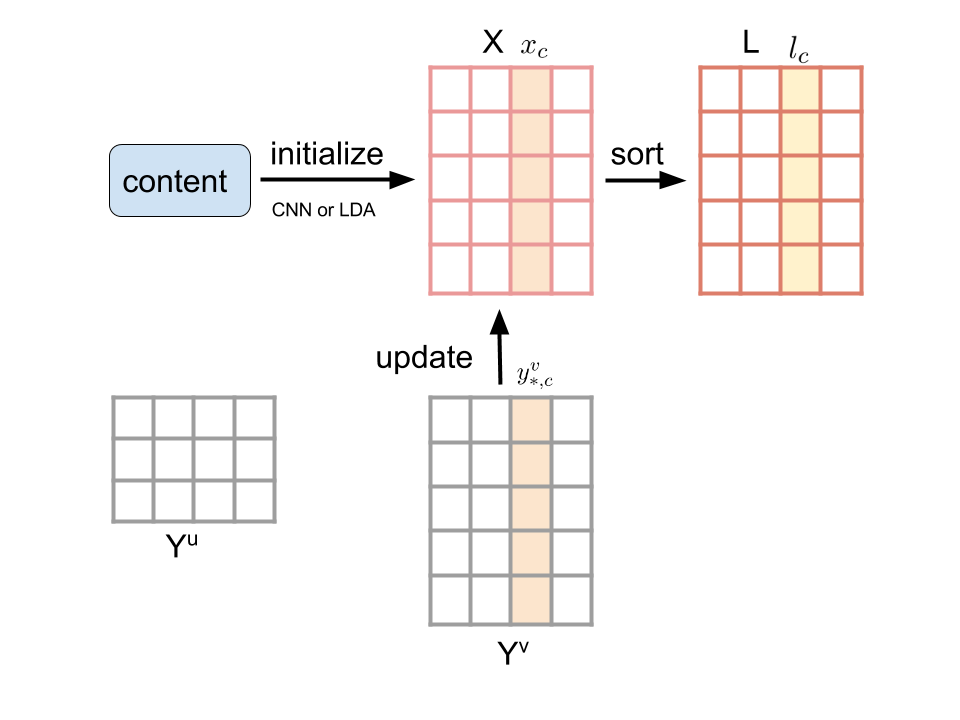
\includegraphics[width=3.5in]{algo2}
	%	\end{center}
	\caption{Adaptive sampling algorithm}
	\end{figure}
\end{frame}


\begin{frame}{Adaptive sampling algorithm}
	\IncMargin{1em}
	\begin{algorithm}[H]%Beamer中的算法排版需要加选项[H]以解决浮动环境问题​
		\SetAlgoNoLine %不要算法中的竖线
		Draw a popular category $c$ from $p\left(c|\rho\right)$\;
		\If {$sim \left(x_c,y_{*,c}^v\right) > \delta $}{
			Update $x_c$ by $y_{*,c}^v$\;
			Reorder items under $c$ and update $l_c$\;
		}
		Draw $\left(u_m,v_i\right) \in \mathcal{P}$ uniformly\;
		Draw a category $c$ from $p\left(c|u_m,v_i\right)$,$\left(1\leq c \leq k\right)$\;
		$\rho_c ++$\;
		Draw a rank $r$ from $p\left(r\right) \propto exp\left(-r/\lambda\right),\left(1\leq c \leq k\right)$\;
		$v_j \leftarrow 
		\begin{cases}
		index\left(c,r\right) & if \ sgn\left(y_{m,c}^u\right) = 1\\
		index\left(c,n-r-1\right) & else
		\end{cases}$\;
		\caption{Content-aware and Adaptive sampling}
		\label{algo:sampling}
	\end{algorithm}
	\DecMargin{1em}
\end{frame}



